\documentclass{IEEEtran}

% Your packages
\usepackage{graphicx}
\usepackage[utf8]{inputenc}
\usepackage[T1]{fontenc}
\usepackage{xcolor}
\usepackage{multirow}
\usepackage{float}
\usepackage{subfigure} % Side by side figures
\usepackage{amsmath}
\usepackage{booktabs}
\usepackage{hyperref} % Has to be the last package imported
\usepackage{algorithm}
\usepackage{algpseudocode}
\usepackage{biblatex} % Imports biblatex package
\addbibresource{biblio.bib} % Import the bibliography file

\begin{document}
	
	\newcommand{\redd}[1]{{\color{red}#1}}
	
	\title{\LARGE \bf
		Visual Recognition \\
		{\small Object Detection, Recognition and Segmentation}
	}
	
	\author{ \parbox{4 in}{\centering Aleix Pujol, Diana Tat, Georg Herodes, Gunjan Paul\\
			Master in Computer Vision\\}
	}
	
	%\author{Aleix Pujol, Diana Tat, Georg Herodes, Gunjan Paul}
	
	\maketitle
	
	\thispagestyle{empty}
	\pagestyle{empty}
	
	
	%%%%%%%%%%%%%%%%%%%%%%%%%%%%%%%%%%%%%%%%%%%%%%%%%%%%%%%%%%%%%%%%%%%%%%%%%%%%%%%%
	\begin{abstract}
		This week came with the challenge of working with the Detectron2 framework and understanding how to deal with annotation formats. We have applied Faster R-CNN and Mask R-CNN models to track and segment the cars and pedestrians, using the KITTI-MOTS dataset and COCO weights. We have also tried the newest version of YOLO v9 and see its performance. 
	\end{abstract}
	
	
	%%%%%%%%%%%%%%%%%%%%%%%%%%%%%%%%%%%%%%%%%%%%%%%%%%%%%%%%%%%%%%%%%%%%%%%%%%%%%%%%
	\section{Introduction}
	During this task we have used PyTorch to implement our neural network and Detectron2 for an efficient object detection
	PyTorch is a very adaptive and dynamic method of building models. Because of that, we can modify and debug the code easy, as well as transform it to PyTorch Lightning. On the other hand, Keras, has a more high-level abstraction  and computational graphs that facilitate the efficient deployment and optimisation of the code.
	
	This week we have been using Detectron2 framework which is made by Facebook Artificial Intelligence Research's. It is based on PyTorch and it features panoptic segmentation, bounding box and instance segmentation mask object recognition. It provides a wide range of models, such as Panoptic FPN, Dense Pose, TensorMask and the ones that we focused on, Mask R-CNN and Faster R-CNN. 
	
	Faster R-CNN provides accurate object localisation by using Region of Interest (RoI) pooling. It suggest regions for examination and then it uses Convolutional Neural Networks (CNNs) to extract the information, simplifying the detection process. Faster R-CNN produces generally accurate object localisation, but it can’t work with masks, which are useful in situations when we need more precise information of the object boundaries. For this reason, Mask R-CNN was introduces as an extension of Faster R-CNN. It overcomes its drawback by having an extra branch that is responsible for segmenting the prediction mask. It uses pixel-wise segmentation and it more precisley in object identification.
	
	Also, as an optional task we have tried the new version of YOLO, YOLO v9. YOLO is an algorithm that performs real-time object detection by  dividing the image into a grid and predicting bounding boxes and class probabilities. We have evaluated and compared its performance with the Faster R-CNN and Mask R-CNN models. 
	
	\section{Related Works}
	
	\subsection{Neural Networks in Computer Vision}
	In the field of computer vision, as \cite{DLinCVReview} says, deep learning has become indispensable for how machines perceive and process visual data. Convolutional neural networks (CNNs), in particular, are deep learning models that have demonstrated unmatched performance in tasks like object detection, instance segmentation, and image categorization. They are able to recognise complex patterns and features, going beyond conventional computer vision techniques, thanks to their autonomous learning of hierarchical representations from unprocessed visual data.
	
	\subsection{Object Detection}
	\subsubsection{Objectives and Uses}
	%reviews
	Deep learning has brought to an important shift in object detection, a fundamental aspect of computer vision. In important studies like Zhao et al.'s \cite{ObjDetReview} from 2018, the writers thoroughly examine this paradigm change by diving into the complexities of object detection enabled by deep learning techniques. A more recent study, published in 2020 by Xiao et al. \cite{ObjDetReview2}, offers a modern viewpoint by showcasing the developments in deep learning-based object identification and its numerous uses in multimedia tools and applications. Moreover, Kaur and Singh's paper \cite{ObjDetReview3} from 2023 provides a thorough examination, highlighting how object detection is changing in the context of digital signal processing. 
	
	
	\subsubsection{Two-Shot Detectors}
	%rcnns
	Two-Shot Detectors are an important advance in the field of object detection since they enable more precise and nuanced identification of visual objects. 2015 saw the introduction of Faster R-CNN\cite{fastrcnn}. By integrating region proposal networks, this paper study transformed object identification and greatly enhanced real-time performance. The Faster R-CNN framework built on this basis to create the framework for later advancements in two-shot detection techniques.
	
	One key illustration of this trajectory's evolution is the Faster Mask R-CNN refinement by Ren et al. \cite{fasterrcnn} that same year. This iteration presents Region Proposal Networks (RPNs), which are meant to make region proposals more quickly and efficiently while also accelerating the object detection process. These Two-Shot Detectors are very useful in improving the accuracy of object detection and laying the groundwork for future improvements like the incorporation of instance segmentation as shown by Mask R-CNN \cite{maskrcnn}. This is especially true of Faster R-CNN and its variants.
	
	With the introduction of Mask R-CNN in \cite{maskrcnn}, instance segmentation has made substantial progress. This model adds a second branch to the Faster R-CNN architecture, which predicts segmentation masks in addition to bounding boxes and class labels. Mask R-CNN works by first producing region suggestions, which it then refines to provide precise object masks. A critical layer of information is added by integrating pixel-level segmentation, which allows the model to offer detailed spatial awareness of object instances inside an image.
	
	\subsubsection{Single-Shot Detectors}
	In the field of object detection, single-shot detectors (SSDs) have become an important category because they provide real-time processing capabilities without sacrificing accuracy.
	
	The YOLO series of single-shot detectors, initially developed and iterated upon by Redmon and Farhadi in \cite{yolov1}, \cite{yolov2}, \cite{yolov3} employs methods such as a grid-based approach and the prediction of bounding boxes as deviations of anchor boxes to provide single-pass detection capabilities. This method has been extensively improved by various researchers in both indurtry and academia. The most recent updates such as YOLOv7 \cite{yolov7}, and most recently, YOLOv9 \cite{yolov9} enhance the performance of single shot detectors even further by optimizing not only the network architecture but also introduce and apply methods such as ELAN, GELAN, and PGI to the training process to overcome issues such as the information bottleneck and inefficient parameter utilization\cite{yolov7}\cite{yolov9}. Such improvements have made the more recent versions of YOLO not only faster, but also more accurate than their predecessors which removes the need to trade off speed or accuracy when choosing a model architecture for object detection. 
	
	\begin{figure}
		\centering
		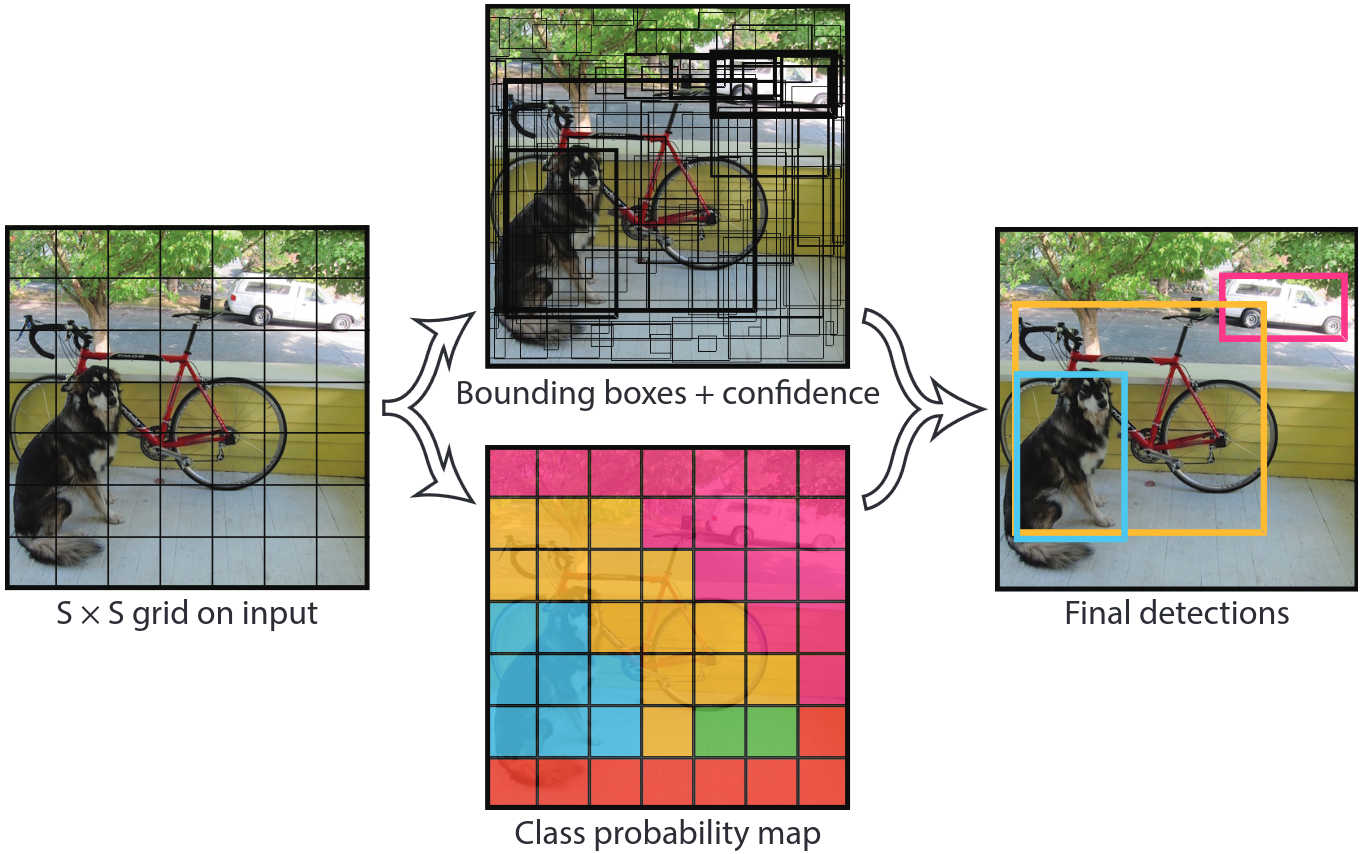
\includegraphics[width=0.8\linewidth]{images/yolo_detect_viz.png}
		\caption{YOLO models represent detection as a regression problem by dividing the image into a grid and predicting classes, bounding box coordinates, and confidences for each cell in the grid \cite{yolov1}}
		\label{fig:yolo_viz}
	\end{figure}
	
	\subsubsection{Segmentation}
	In computer vision segmentation is important because it allows to understand the input data better. A in depth analysis of object detection using deep learning for segmentation is explained in \cite{segm1}, enhancing the precision of the segmentation results. In the paper \cite{segm2} the focus is on exploring different models and approaches, highlighting the effectiveness of trying different methods and their applicability in different contexts. Furthermore, \cite{segm3} provides an examination of object detection using deep learning in the context of digital signal processing, illuminating the significant developments and difficulties in the area.
	
	\subsubsection{RetinaNET}
	RetinaNet, as \cite{RetinaNet}, is an object detection method that tackles the complexities involved in identifying objects of different sizes, particularly small and overlapping ones. The research paper focuses on addressing the challenges commonly found in object detection approaches. A notable aspect of this work is the introduction of the focal loss mechanism, which involves adjusting the weight of training samples. This strategy enables the model to prioritise instances during training leading to performance in detecting complex objects. Additionally RetinaNet incorporates a Feature Pyramid Network (FPN) that effectively captures features at scales proving essential for handling objects with dimensions. The combination of loss and FPN sets RetinaNet apart. Helps it achieve outstanding results, in practical object detection scenarios.
	
	\subsubsection{DETR}
	DETR (End, to End Object Detection with Transformers) represents a step in the realm of object detection. The study \cite{DETR} introduces a method for detecting objects by using transformer architectures. In contrast to other techniques, DETR directly forecasts object queries and their positions removing the necessity for anchor boxes and non maximum suppression. This comprehensive framework simplifies the detection process. Tackles the challenges associated with object sizes and overlaps. The research highlights DETRs capacity to redefine how object detection is approached, delivering localisation and classification outcomes. It showcases the effectiveness of transformer models in tasks related to computer vision signalling a shift, from methodologies.
	
	\subsection{Object Detection}
	\subsubsection{Objectives and Uses}
	%reviews
	Deep learning has brought an important shift in object detection, a fundamental aspect of computer vision. In important studies like Zhao et al.'s \cite{ObjDetReview} from 2018, the writers thoroughly examine this paradigm change by diving into the complexities of object detection enabled by deep learning techniques. A more recent study, published in 2020 by Xiao et al. \cite{ObjDetReview2}, offers a modern viewpoint by showcasing the developments in deep learning-based object identification and its numerous uses in multimedia tools and applications. Moreover, Kaur and Singh's paper \cite{ObjDetReview3} from 2023 provides a thorough examination, highlighting how object detection is changing in the context of digital signal processing. 
	
	\section{Methodology}
	\subsubsection{Faster-R-CNN}
	Faster R-CNN works by initial removing distinct attributes from the input photo making use of a distinct neural network (CNN) foundation such as ResNet or VGG. These functions are after that fed right into both the RPN coupled with a region-based discovery network.
	
	The RPN runs by moving a tiny network normally a couple of distinct layers over the function map creating a collection of area propositions. These propositions include bounding boxes and also linked objectness ratings, showing the probability of having a things. The RPN is educated end-to-end to create premium area propositions effectively.
	
	During training, the Faster-R-CNN model is trained end-to-end using a multi-task loss function that combines classification and regression losses. We employ a stochastic gradient descent (SGD) optimiser with momentum to minimise the loss function and update the network parameters.
	
	In our experiments, we fine-tune a pre-trained Faster-R-CNN model on our dataset, which consists of images annotated with object bounding boxes. We evaluate the performance of the trained model using standard metrics such as mean Average Precision (mAP) and compare it against baseline methods and other state-of-the-art object detection frameworks.
	
	\subsubsection{Mask-R-CNN}
	
	Mask R-CNN extends Faster R-CNN by integrating a totally convolutional network (FCN) branch together with the existing area proposition network (RPN) as well as region-based discovery network. This FCN branch produces division masks for recommended areas allowing pixel-level division within pictures. Unlike Faster R-CNN which concentrates exclusively on bounding box forecast, Mask R-CNN incorporates things discovery and also circumstances division jobs in an unified style making it ideal for jobs needing exact things limit circulation. Throughout training both designs maximise multi-task loss features consisting of category as well as bounding box regression losses, yet Mask R-CNN includes a mask forecast loss to educate the division mask generation branch.
	
	During training, the Mask-R-CNN model is trained end-to-end using a multi-task loss function that combines classification, bounding box regression, and mask prediction losses. Similar to Faster-R-CNN employ a stochastic gradient descent (SGD) optimiser with momentum to minimise the loss function and update the network parameters.
	
	In our experiments, we fine-tune a pre-trained Mask-R-CNN model on our dataset, which consists of images annotated with object bounding boxes and instance segmentation masks. We evaluate the performance of the trained model using standard metrics such as mean Average Precision (mAP) at various thresholds.
	
	We can see that Mask R-CNN and Faster R-CNN for feature extraction have a same backbone, ResNet50, in Figure~\ref{fig:faster_mask_rcnn}. Both of them have a Region of Interest (RoI) pooling layer for feature extraction from these proposals and a Region Proposal Network (RPN) for generating region proposals. Nonetheless, the "ROI Head" element of the networks accounts for the majority of the differences. The ROI Head in Faster R-CNN is made up of sub-networks for bounding box regression and object classification. On the other hand, Mask R-CNN builds upon Faster R-CNN by incorporating a second sub-network for mask prediction, which allows it to execute instance segmentation in addition to object detection. 


	
	\begin{figure}[htbp]
		\centering
		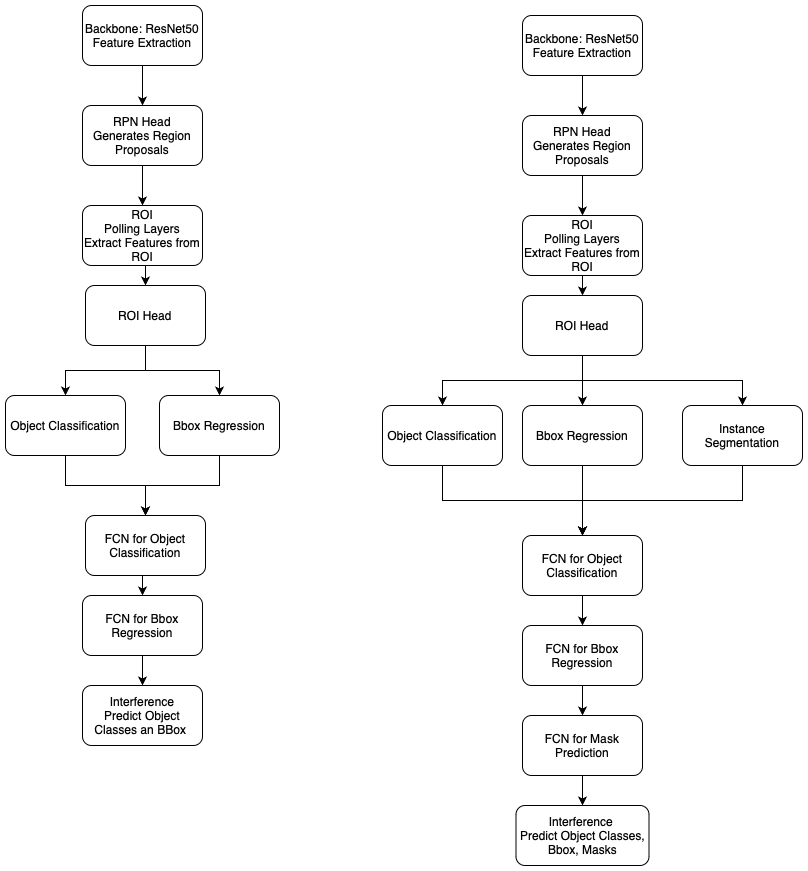
\includegraphics[width=0.5\textwidth]{images/faster_mask_rcnn.png}
		\caption{Architecture of Faster R-CNN(a) and Mask R-CNN(b).}
		\label{fig:faster_mask_rcnn}
	\end{figure}
	
	
	\subsubsection{YOLOv9}
	As an example of a newer SOTA object detection model we employ YOLOv9, an evolution of the YOLO (You Only Look Once) object detection framework, for our object detection task. YOLOv9 builds upon the principles of the YOLOv7 architecture while introducing several key improvements to enhance both accuracy and speed. Such as extending the ELAN method proposed in the YOLOv7 paper to create GELAN, as well as by introducing a new concept called Programmable Gradient Information.
	
	One substantial addition in YOLOv9 is the expansion of the ELAN (Reliable and also Light-weight Anchor-free Network) approach recommended in the YOLOv7 paper, causing GELAN (International Extremum Learning-based Anchor-free Network) GELAN enhances the performance of item discovery by efficiently taking care of range variants and also things localisation precision. Additionally, YOLOv9 presents an unique principle called Programmable Gradient Information which better improves the version's capacity to discover things with high accuracy.
	
	During training, YOLOv9 is trained end-to-end using a combination of localisation loss, confidence loss, and class probability loss. The model is optimised using the ADAM optimiser with techniques such as learning rate scheduling and momentum to improve convergence and stability. As is common with newer YOLO models, aggressive augmentation techniques such as mosaicing and color jitter are used in the training process to increase model robustness to noise, scaling and translation.
	
	In our experiments, we fine-tune a pre-trained YOLOv9 model on our dataset, which consists of images annotated with object bounding boxes. We evaluate the performance of the trained model using standard metrics such as mean Average Precision (mAP) and Intersection over union(IoU).
	
	We can observe the model architecture of YOLOV9 in the image \ref{fig:yolov9_architecture}. It predicts bounding boxes and class probabilities for each grid cell by first splitting the input image into a grid. A backbone network for feature extraction—typically Darknet or a comparable architecture—makes up the YOLOv9 architecture. Additionally, it has several detecting heads at varying scales, which enables the model to effectively recognise objects with a range of sizes and aspect ratios. Compared to two-stage detectors like Faster R-CNN, YOLOv9 is faster and more suited for real-time applications because it uses a single-stage architecture. Furthermore, YOLOv9 offers a number of enhancements over its predecessors, such as improved training procedures and feature pyramid networks (FPN), which lead to better detection performance. All things considered, YOLOv9 provides a speed and accuracy balance that makes it a popular option for object detection jobs in a variety of areas.
	
	\begin{figure}[htbp]
		\centering
		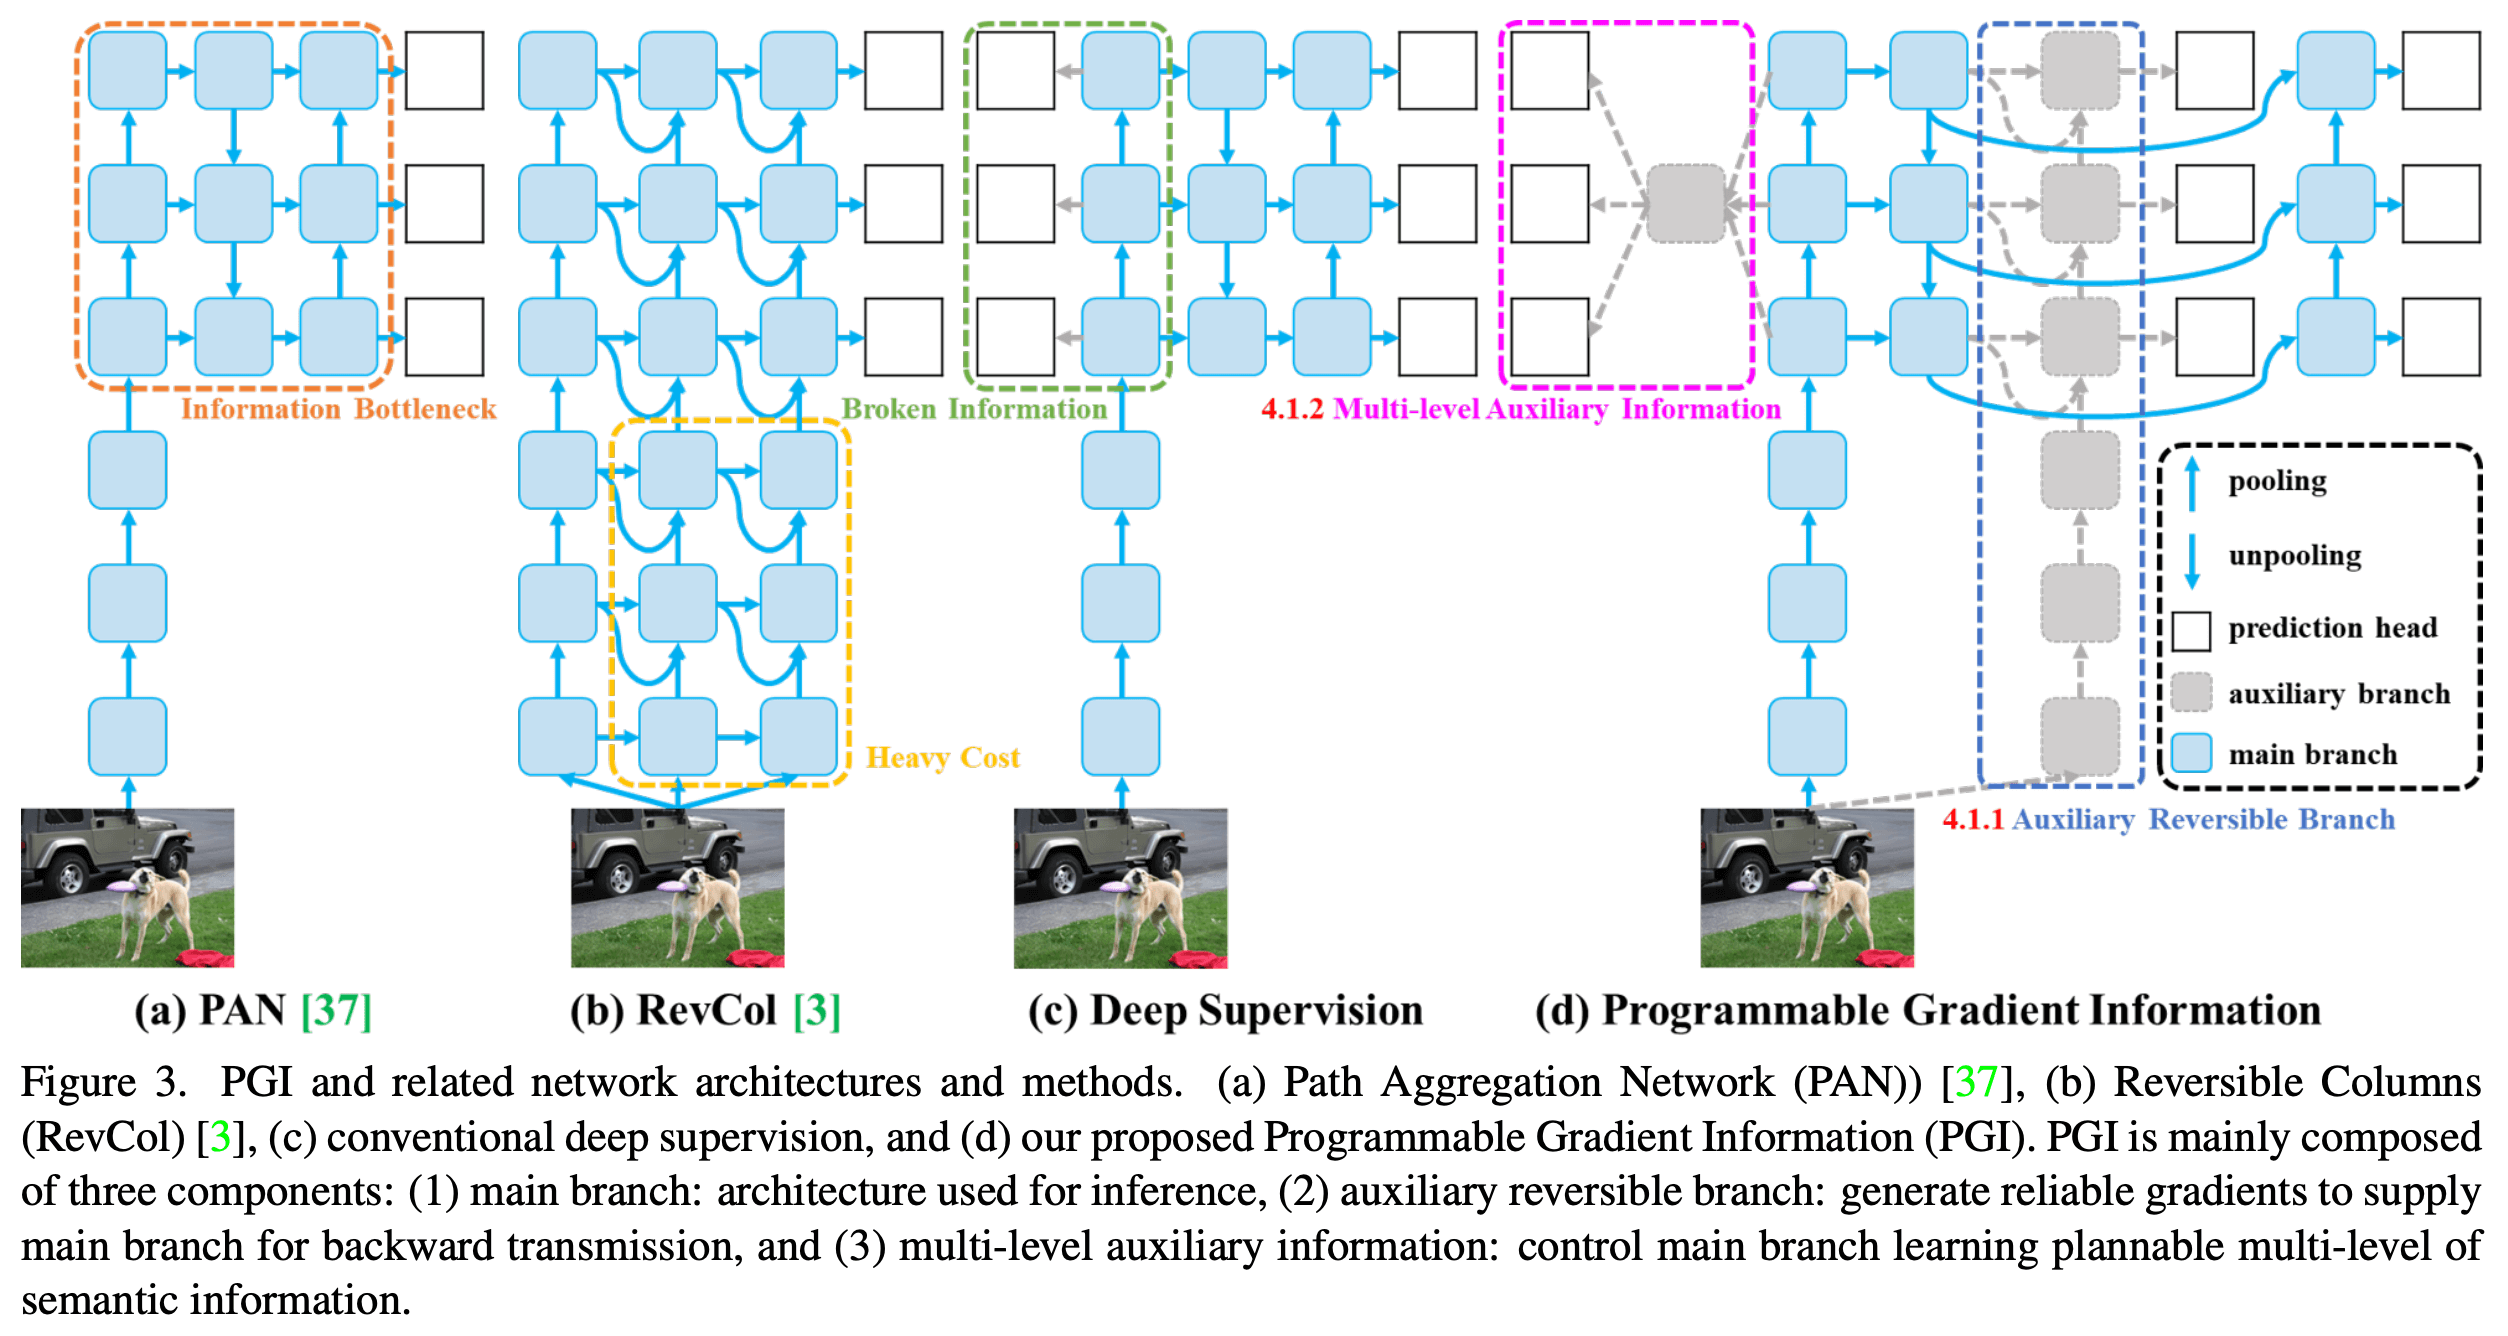
\includegraphics[width=0.5\textwidth]{images/yolov9.png}
		\caption{Architecture of YOLOv9. Source: \textit{YOLOv9: Ultralytics' YOLOv5 Implementation}~\cite{ultralytics_yolov9}}
		\label{fig:yolov9_architecture}
	\end{figure}

	
	In Figure~\ref{fig:yolov9_architecture}, we can see the architecture of YOLOv9, which stands for You Only Look Once version 9. YOLOv9 is a state-of-the-art object detection algorithm that operates by dividing the input image into a grid and predicting bounding boxes and class probabilities for each grid cell. The YOLOv9 architecture consists of a backbone network, typically Darknet or a similar architecture, for feature extraction. It further includes multiple detection heads at different scales, allowing the model to detect objects of various sizes and aspect ratios efficiently. YOLOv9 employs a single-stage architecture, making it faster and more suitable for real-time applications compared to two-stage detectors like Faster R-CNN. Additionally, YOLOv9 introduces several improvements over its predecessors, including feature pyramid networks (FPN) and enhanced training strategies, resulting in superior detection performance. Overall, YOLOv9 offers a balance between speed and accuracy, making it a popular choice for object detection tasks across various domains.
	
	
	\section{Experimental design}
	\subsubsection{Dataset: KITTI-MOTS}
	
	The dataset includes a collection of training sequences totalling 12, which contain 8,073 pedestrian masks and 18,831 annotated car masks. The validation set is made up of 9 sequences with 3,347 pedestrian masks and 8,068 car masks. Additionally there are 29 sequences specifically reserved for testing. For labelling instances cars are labeled in order starting from 1000 onwards while pedestrians follow a similar pattern starting from 2000.
	We can observe how a frame from the dataset looks like in figures \ref{fig:kitti_dataset}.
	
	\begin{figure}
		\centering
		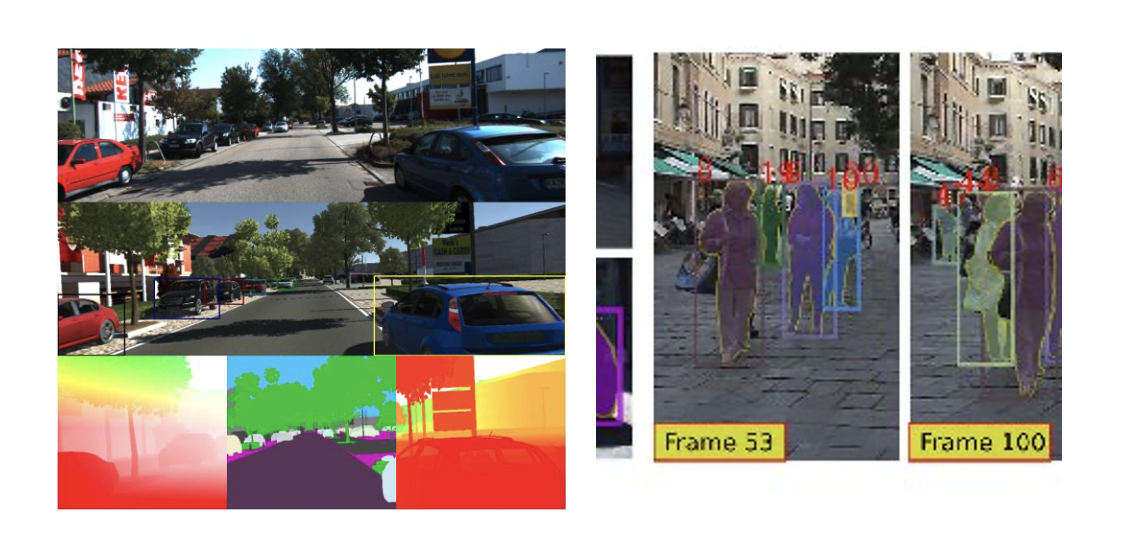
\includegraphics[width=0.8\linewidth]{images/kitti_dataset.png}
		\caption{KITTI MOTS Dataset(left) and Annotations(right).}
		\label{fig:kitti_dataset}
	\end{figure}
	
	\subsubsection{Metrics}
	\paragraph{Overview}
	For the evaluation of our code, we have use Precision, Recall, F1,  AP
	AP@50 and mAP@75.
	
	Mean Average Precision, at k (mAP@k) assesses the balance between precision and recall focusing on the precision when considering the top k predictions for each image. It involves calculating the precision for each query based on the relevance of predictions within the top k. 
	\[ \text{MAP@k} = \frac{1}{|Q|} \sum_{q \in Q} \left( \sum_{i=1}^{k} \frac{\text{Precision}@i \cdot \text{relevant}_{q,i}}{i} \right) \]
	
	Precision measures how accurately the model identifies objects by comparing true positive predictions to all predicted positives. 
	
	Recall indicates the models ability to detect all objects by comparing positives to all actual positives. 
	\[
	\text{Precision} = \frac{\text{TP(True Positive)}}{\text{TP(True Positive) + FP(False Positive)}}
	\] 
	
	Intersection over Union (IoU) is used to determine how much two bounding boxes predicted and ground truth behind them overlap, which enables one to get an idea of the object localisation accuracy by assessing intersection and union areas of these boxes. 
	This helps in determining if a prediction was a true positive, (TP), a false positive (FP), or a false negative, (FN) depending on the overlap that occurs between the predicted box and the ground truth box. 
	
	\[
	\text{IoU} = \frac{\text{Area of Intersection}}{\text{Area of Union}} = \frac{\text{TP}}{\text{TP + FP + FN}}
	\]
	
	The F1 Score combines Precision and Recall while AP is calculated by integrating over different IoU thresholds under the precision-recall curve. Its influence shows how much IoU contributes in evaluating object detection model effectiveness since it gives information about detection accuracy as well as localisation capability.
	
	\[
	F1 = \frac{2 \times \text{Precision} \times \text{Recall}}{\text{Precision} + \text{Recall}}
	\]
	
	Together, these metrics provide a framework for evaluating the effectiveness of object detection models.
	
	\paragraph{Code evaluation}
	In case of  \textbf{Faster R-CNN} we have evaluated the architecture, including its convolutional layers, RPN, and R-CNN for object detection. The model was fine-tuned using our dataset, with careful adjustments made to hyper-parameters such as learning rates and batch sizes for optimal performance. We have constantly monitored the model's training progress to ensured convergence and prevent the overfitting. We have tested it on a separate validation dataset, assessing precision, recall, and mAP scores across various object classes. In addition, we have extracted some qualitative analysis to identify potential weaknesses and areas for improvement.
	
	Similarly, we evaluated the \textbf{Mask R-CNN} for instance segmentation, including its FPN, RPN, and mask prediction head. By conducting hyper-parameter tuning experiments, we optimised the model for our specific task, exploring different learning rates, weight decay values, and augmentation techniques. We have evaluated the model's performance on segmentation and object detection tasks, analyzing accuracy, IoU scores, and mAP across different object categories.
	
	\textbf{YOLOv9} was evaluated for real-time object detection. The emphasis was on its single CNN architecture, with a focus on balancing speed and accuracy. We have conducted extensive exploration of model configurations and fine-tuning parameters, considering dataset characteristics and augmentation during training. In addition to traditional metrics, real-time processing capabilities were assessed against speed benchmarks. The evaluation provided deep insights into YOLOv9's strengths and limitations for diverse object detection tasks.
	
	\subsubsection{Implementation details}
	\paragraph{Faster R-CNN}
	We used PyTorch and Detectron2 for our Faster R-CNN implementation. The first step we took was to define the structure of the model and load pre-trained weights from the COCO dataset. We optimised performance by setting parameter like score threshold for predicting instances. For this purpose, we developed a function that loads images for testing on custom datasets and converts annotations into the COCO format using $convert_to_coco$ function. This involved extracting bounding box coordinates and class labels as well as converting coordinates to $XYXY_ABS$ format so as to ensure compatibility with Detectron2. After that, we saved the COCO dataset into a JSON file that could be employed in either training or evaluation purposes. Then, using an adjusted configuration, we created a Faster R-CNN predictor which could perform inference on test images. The Visualizer component visualised detection outcomes by superimposing bounding boxes and class labels onto input images for easier interpretation.
	
	\begin{figure}[htbp]
		\centering
		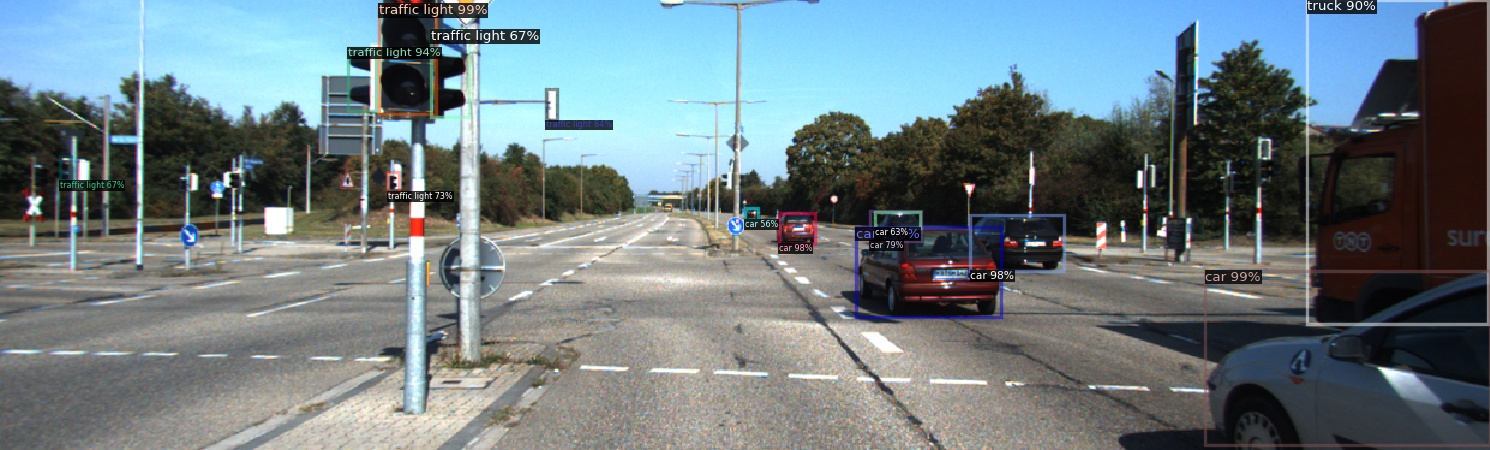
\includegraphics[width=0.5\textwidth]{images/faster_inferred_image.jpg}
		\caption{Faster R-CNN Inferred Image}
		\label{fig:faster_inferred_image}
	\end{figure}
	
	Afterwards we stored the visualized image in a file, which enabled us to analyze it and share the detection results. This method shows how efficiently we used trained object detection models from Detectron2 to make inferences on custom datasets proving how well Faster R CNN works, in practical situations.
	
	\textbf{Fine-Tuning Faster R-CNN}
	After loading the model with the KITTI MOTS dataset, we moved to the next step of fine-tuning that model to both the domain and the task under test. To start with, we used the trained Faster R-CNN model with an R50 FPN backbone and 3x training duration as the starting point. During the retraining process we refined the hyperparameters in order to improve the models efficacy. This was done by training batch of 32 for 400 epochs and adjusting batch size per image to 128. Besides that, we looked through how different learning rates affected the model performance by checking outcomes on the test set.
	
	\paragraph{Mask R-CNN}
	For Mask R-CNN the same approach was adopted to implement the model with all the required parameters and pre-trained weights from the COCO dataset. We used the R50-FPN architecture with a 3x training schedule. To ensure the reliability of our model's outputs we set the threshold limit for instance predictions. In contrast with Faster R-CNN, Mask R-CNN needs both images and masks as input for the segmentation of the pixel level. This leads to modifications in data format and mask annotation during preprocessing phase. Despite the modifications in the procedure, mask annotations came in addition to the bounding boxes. Moreover, when loading data, bounding box coordinates and mask attributes were also parsed and applied to the dataset, guaranteeing that the model received both image and mask data as input.
	
	As before, we have created a visualizer instance that contains bounding boxes and maks, as we can see in the images \ref{fig:mask_sample} and \ref{fig:mask_interf_output}  . 
	
	\begin{figure}[htbp]
		\centering
		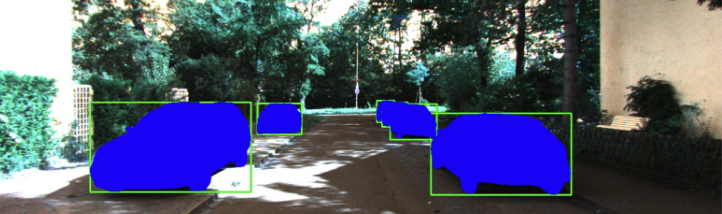
\includegraphics[width=0.5\textwidth]{images/mask_sample.png} 
		\caption{Training KITTI-MOTS sample used for inference}
		\label{fig:mask_sample}
	\end{figure}
	
	\begin{figure}[htbp]
		\centering
		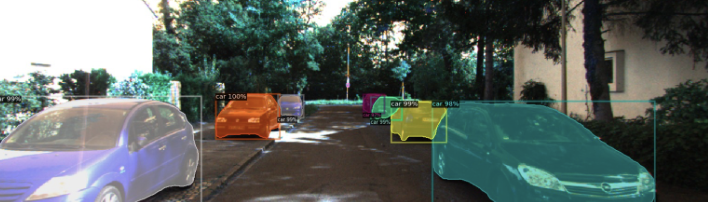
\includegraphics[width=0.5\textwidth]{images/mask_interf_output.png} 
		\caption{Inference output case}
		\label{fig:mask_interf_output}
	\end{figure}
	
	In general, Mask R-CNN was implemented using the same approach as for Faster R-CNN, the only differences being the input information.
	
	\paragraph{YOLOv9}
	For the optional task we have used the new YOLOv9 algorithm. We start by placing the images in directories with their matching ground truth and labels. Then we are converting the bounding box coordinated from YOLO format to $XYXY$ which allows a consistent visualisation and easy of interpretation. Next we analyse each image and retrieve its dimensions in order to get the precise bounding box location. The text files annotations are parsed to get the bounding box coordinates and class IDs. 
	
	We can’t say a lot about the implementation details, because it was already been implemented so we focused on fine-tuning it and see its performance on the person and car classes in the dataset. We have used fine-tuned the weights that were adjusted after being training on the COCO dataset. 
	
	This shows us that even though the model performs good when it comes to bigger objects, it fails to detect the small ones, as we can see in \ref{fig:yolo_predictions} and \ref{fig:yolo_gt}. We discovered that the class 10 objects in the KITTI-MOTS dataset might be be annotated to potentially resolve inconsistencies because their absence would affect the overall performance.
	
	\begin{figure}[htbp]
		\centering
		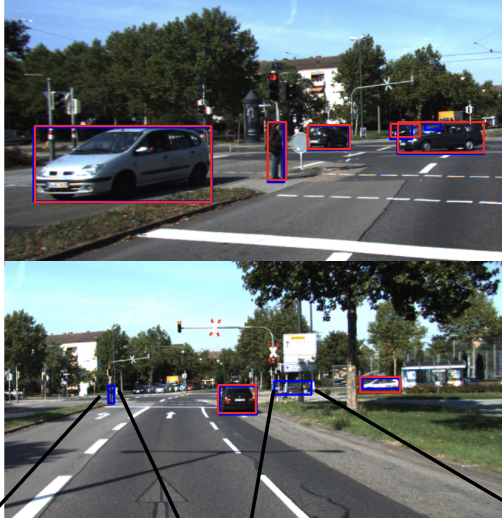
\includegraphics[width=0.4\textwidth]{images/yolo_1.png} 
		\caption{YOLOv9 Predictions (red)}
		\label{fig:yolo_predictions}
	\end{figure}
	
	\begin{figure}[htbp]
		\centering
		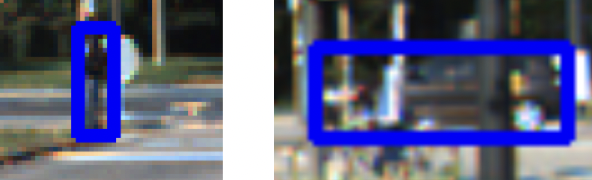
\includegraphics[width=0.4\textwidth]{images/yolo_2.png} 
		\caption{YOLOv9 Ground Truth (blue)}
		\label{fig:yolo_gt}
	\end{figure}
	
	\section{Results}
	
	Upon evaluating the pre-trained Faster R-CNN version's efficiency on the KITTI MOTS examination information collection, it attained a Precision of 0.4191 Recall of 0.5702 and also F1 Score of 0.4629 as displayed in table \ref{tab:overall_metrics}. We have observed some difficulties particularly with the "Pedestrian" classification, where we have obtained a precision of 0.1876 was observed, which can be seen in \ref{tab:class_metrics}. This concern originated from circumstances where the version inaccurately recognized obstacles as pedestrians  a result of visual resemblances stressing the requirement for precision enhancement in real-world circumstances.
	
	\begin{table}[h]
		\centering
		\begin{tabular}{lccc}
			\toprule
			Metric & Precision & Recall & F1 Score \\
			\midrule
			Overall & 0.4191 & 0.5702 & 0.4629 \\
			\bottomrule
		\end{tabular}
		\caption{Overall Metrics}
		\label{tab:overall_metrics} 
	\end{table}
	
	\begin{table}[ht]
		\centering
		\begin{tabular}{lcccc}
			\toprule
			Class & Precision/Recall/F1 & AP & AP@50 & mAP@75 \\
			\midrule
			Pedestrian & 0.1876 / 0.2769 / 0.2104 & 0.1876 & 9.9139 & 6.6093 \\
			Car & 0.6505 / 0.8636 / 0.7155 & 0.6505 & 34.3741 & 22.9161 \\
			\bottomrule
		\end{tabular}
		\caption{Class-wise Metrics}
		\label{tab:class_metrics}
	\end{table}
	
	The examination outcomes of the Mask R-CNN on the KITTI-MOTS information, summarised in Table \ref{tab:mask_rcnn_results}, highlighted its efficiency in pixel-level division, particularly with an mAP of 44.23\% for cars together with 21.76\% for pedestrians. The particular metrics such as AP@50 as well as mAP@75 offered understandings right into the design's precision at various IoU limits, showcasing its strength throughout numerous circumstances.
	
	
	\begin{table}[ht]
		\centering
		\begin{tabular}{lccc}
			\toprule
			Class & mAP & AP@50 & mAP@75 \\
			\midrule
			Pedestrian & 21.76 & 14.756 & 8.633 \\
			Car & 44.23 & 37.651 & 24.651 \\
			\bottomrule
		\end{tabular}
		\caption{Mask R-CNN Evaluation Results on KITTI-MOTS}
		\label{tab:mask_rcnn_results}
	\end{table}
	
	In the case of Faster R-CNN, we experimented with different learning rates, aiming to strike a balance between precision and computational efficiency. Our results, as shown in Table \ref{tab:faster_learning_rate_performance}, underscore the importance of careful hyperparameter tuning in achieving optimal performance. 
	
	\begin{table}[H]
		\centering
		\small
		\begin{tabular}{@{}cccccc@{}}
			\toprule
			\textbf{LR} & \textbf{mAP} & \textbf{mAP@50} & \textbf{Car mAP} & \textbf{Pedestrian mAP} & \textbf{Time} \\ \midrule
			0.0025 & 13.171 & 32.268 & 13.046 & 6.721 & 39 ms \\
			0.01 & 45.323 & 75.034 & 53.506 & 28.025 & 38 ms \\
			0.025 & 46.636 & 78.035 & 52.961 & 32.304 & 41 ms \\ \bottomrule
		\end{tabular}
		\caption{Effect of learning rate on Faster R-CNN training}
		\label{tab:faster_learning_rate_performance}
	\end{table}
	
	
	Similarly, for Mask R-CNN, fine-tuning with the ResNet-50-FPN architecture and a three-time training schedule yielded slight improvements in mAP for both bounding box detection and pixel-level segmentation tasks, as demonstrated in Table \ref{tab:mask_test_bounding_box_evaluation}.
	
	\begin{table}[H]
		\centering
		\begin{tabular}{@{}cccccc@{}}
			\toprule
			\textbf{LR} & \textbf{mAP} & \textbf{mAP@50} & \textbf{Car mAP} & \textbf{Pedestrian mAP} & \textbf{Time} \\ \midrule
			0.025 & 12.781 & 12.791 & 5.479 & 1.670 & 55 ms \\
			0.1 & 13.180 & 13.353 & 5.257 & 1.660 & 55 ms \\ \bottomrule
		\end{tabular}
		\caption{Evaluation results for bounding box detection on the test set}
		\label{tab:mask_test_bounding_box_evaluation}
	\end{table}
	
	For YOLOv9, our emphasis got on boosting discovery precision with fine-tuning. In spite of very little renovations in mAP50, we observed that comprehensive calibration as well as specification modification were important for taking on real-world difficulties efficiently. The efficiency contrast of YOLOv9 versions, detailed in Table \ ref{ tab: yolov9}, highlights the requirement for nuanced optimization techniques to accomplish substantial gains in discovery precision.
	
	\begin{table}[H]
		\centering
		\begin{tabular}{@{}cccccc@{}}
			\toprule
			\textbf{Model} & \textbf{mAP50} & \textbf{mAP50:95} & \textbf{Time} \\
			\midrule
			YOLOv9 Pre-trained & 0.838 & 0.593 & 4.8 ms \\
			YOLOv9 Fine-tuned & 0.834 & 0.654 & 4.9 ms \\
			\bottomrule
		\end{tabular}
		\caption{Performance Comparison of YOLOv9 Models}
		\label{tab:yolov9}
	\end{table}
	
	
	\begin{table}[H]
		\centering
		\begin{tabular}{@{}cccccc@{}}
			\toprule
			\textbf{LR} & \textbf{mAP} & \textbf{mAP@50} & \textbf{Car mAP} & \textbf{Pedestrian mAP} & \textbf{Time} \\
			\midrule
			0.025 & 1.421 & 6.094 & 6.506 & 0.000 & 55 ms \\
			0.1 & 5.612 & 0.886 & 6.390 & 0.231 & 55 ms \\
			\bottomrule
		\end{tabular}
		\caption{Segmentation results on the test set}
		\label{tab:mask_test_segm_evaluation}
	\end{table}
	
	On the whole our execution method focused on precise criterion adjusting and also version adjustment to attend to the particular subtleties of the KITTI MOTS information collection. By utilizing the toughness of each version design plus maximizing essential hyperparameters, we intended to optimize efficiency throughout numerous item discovery as well as division jobs eventually adding to innovations in real-world computer system vision applications.
	
	
	\section{Conclusions}
	When comparing the different \textbf{object detection models} we have noticed that Faster R-CNN exhibited robustness, but it faced challenges in crowded or occluded scenarios. Mask R-CNN has improved segmentation, but it still struggles with different urban scenes. For YOLOv9 we noticed some speed capabilities, but again it fails to detect small object accurately. 
	
	In terms of the \textbf{dataset}, dealing with the KITTI-MOTS information, especially concerning annotation layouts as well as information prep work highlights the importance of precise information handling, which can considerably influence the efficiency of things discovery versions together with in circumstances requiring exact division.
	
	We found it more difficult to implement and \textbf{fine-tune} Mask R-CNN than Faster R-CNN. While the algorithm and the approach was more or less the same, we think that the dataset preparation made the difference and it might be a reason why the model struggles to precisely segment pedestrian cases.
	
	\textbf{YOLOv9} clearly outperforms the R-CNN based methods, which is expected as R-CNN-s were SOTA for several years and YOLOv9 is very recent. YOLOv9 struggling with very small objects is expected as that is a common trait of object detection models, especially single shot detectors in general. We kept in mind substantial searching for that highlight the effectiveness of Mask R-CNN in pixel-level division jobs, attaining good results for mAP ratings for both car and pedestrian classes. Furthermore, YOLOv9 was more efficient contrasted to R-CNN-based approaches, especially in identifying smaller sized things, while its concurrent handling abilities and also precision make it a guaranteeing alternative for different things discovery jobs.
	
	In conclusion, even though these models face obstacles including occlusion, crowded scenes, and small item recognition, our research shows how promising these can be in a range of practical applications. For the area of computer vision to grow further, ongoing research efforts focused on improving model architectures, investigating alternative datasets, and tackling new issues will be crucial. Moving forward, if we would explore alternative datasets, and addressing emerging challenges, would be interesting for further advancements in the field of computer vision.
	
	
	
	\nocite{*} % Include all entries from the bibliography file
	
	\printbibliography
	
\end{document}
